\documentclass[12pt,a4paper,UTF8]{article}
% \usepackage{ctex} % Chinese support
\usepackage{graphicx} % Insert images
\usepackage{listings} % Print source code
\usepackage{color} % Color support
\usepackage{booktabs} % Professional table support
\usepackage{pdflscape} % Landscape pages support in PDF
\usepackage{hyperref} % Hypertext links support for cross-referencing

% Customize hyperref format (it's set to no special format here)
\hypersetup{hidelinks}

% Declare directories to search for graphics files for graphicx
\graphicspath{{figures/}{logo/}}

% Define source code style for listings
\lstdefinestyle{python}{
  language=Python,
  basicstyle=\ttfamily\footnotesize,
  keywordstyle=\bfseries\color[rgb]{0, 0, 1},
  identifierstyle=\color[rgb]{0.5, 0.3, 0.1},
  stringstyle=\color[rgb]{0.6, 0.1, 0.1},
  commentstyle=\itshape\color[rgb]{0.05, 0.5, 0.05},
  backgroundcolor=\color[gray]{0.95},
  numbers=left,
  numbersep=5pt,
  numberstyle=\color[gray]{0.6},
  breaklines=true
}

% Define new command for title page
\newcommand{\reporttitle}[2]{
  \LARGE\textsf{#1}\quad\underline{\makebox[12em]{#2}}
}
\newcommand{\reportinfo}[2]{
  \large\makebox[4em]{\textsf{#1}}\quad\underline{\makebox[18em]{#2}}
}

% The document begins here
\begin{document}
\begin{titlepage}
  \centering
  \vspace*{\fill}
  
\includegraphics[height=144pt]{nju-logo}\\[48pt]
  {\huge\textsf{Lab Report}}\\[48pt]
  \reporttitle{Lab Name}{Respond to ICMP}\\[72pt]

  \reportinfo{Course}{Computer Network}\\[8pt]
  \reportinfo{Major}{Computer Science and Technology}\\[8pt]
  \reportinfo{Id}{191220129}\\[8pt]
  \reportinfo{Name}{Shangyu.Xing}\\[8pt]
  \reportinfo{Email}{191220129@smail.nju.edu.cn}\\[8pt]
  \reportinfo{Date}{2021.05}\\
  \vspace*{\fill}
\end{titlepage}

\tableofcontents
\newpage

\section{Objective}
\begin{itemize}
	\item Learn ICMP protocol and how to implement it;
	\item learn to implement hardware logic using the Switchyard framework;
	\item learn to capture network package using wireshark.
\end{itemize}

\section{Requirements}
	This lab requires to implement a router who can respond to ICMP and generate ICMP error messages, in addition to forwarding packets and handling arp requests which was implemented in the last 2 labs. Specifically, the router should do the following:
\begin{itemize}
	\item Respond to ICMP echo requests;
	\item generate ICMP error messages:
	\begin{itemize}
		\item destination network unreachable
		\item time exceeded
		\item destination host unreachable
		\item destination port unreachable
	\end{itemize}
\end{itemize}

\section{Procedure}
I completed all the tasks as required.
In this section, I will explain how I did my work in detail.

\subsection{Modify forwarding logic}
To complete the task, router's forwarding logic implemented in the last lab must be modified.
The logic is below:
\begin{enumerate}
	\item Check if the packet is arp request targeted at the router;
	\item decrease ttl by 1 and generate time exceeded error if reduced to 0 (except that the packet is echo request targeted at the router itself);
	\item if the packet is targeted at the router, check if it is echo request;
	\item if it is, do echo reply; else generate destination port unreachable error;
	\item if the packet is not targeted at the router, forward it.
\end{enumerate}
\lstinputlisting[style=python]{1.py}
During forwarding destination unreachable error can also be generated, so we should do some judgment.
\lstinputlisting[style=python]{2.py}
Lastly, if an arp request is not replied after 5 retries, it should generate destination host unreachable error. This error occurs only when packets in arpQueue (waiting for arp reply) attempt to send arp requests again.
\lstinputlisting[style=python]{3.py}
Now we have successfully constructed the framework for handling ICMP messages.

\subsection{Implementation for ICMP messages}
ICMP message packet consists of 3 headers: Ethernet, IPv4, ICMP. So I created a universal ICMP constructor:
\lstinputlisting[style=python]{4.py}
Next, we should fill in the corresponding data field. We must pay special attention to srcip. \\
For destination unreachable, srcip should be that of the interface which received the packet.
\lstinputlisting[style=python]{5.py}
Note that destination host unreachable is special, because it shouldn't send multiple error messages with the same srcip and dstip even if there are multiple error packets. So I used a set to store all (srcip, dstip) pairs. If it has already sent, just delete the packet from arpQueue without sending error message. \\
For ttl expire, srcip should also be that of the interface which received the packet.
\lstinputlisting[style=python]{6.py}
But for echo reply, srcip should also be the destination specified in the received packet.
\lstinputlisting[style=python]{7.py}

\section{Test \& Result}
\subsection{Testcase}
Firstly I tested my code with switchyard testcases:
\begin{figure}[htbp]
	\centering
	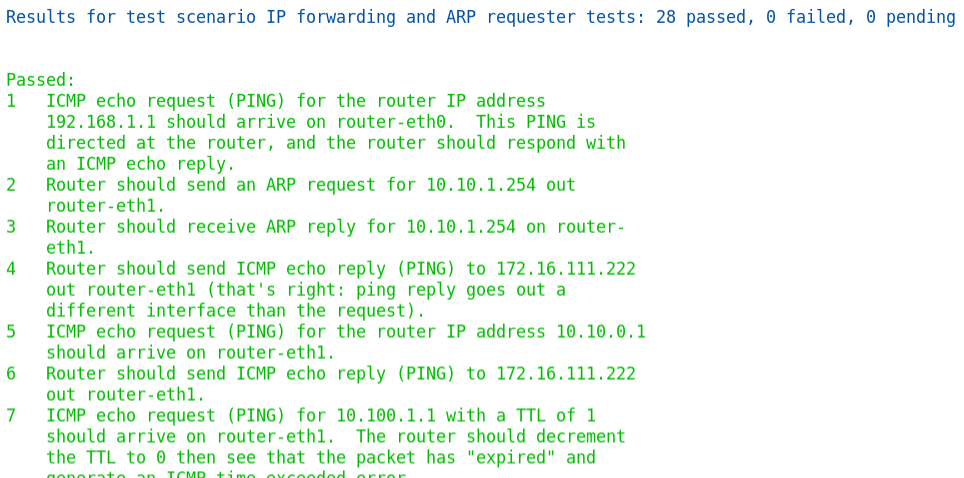
\includegraphics[width=\textwidth]{1}
	\caption{Switchyard test result}
\end{figure}
\newpage

\subsection{Deployment}
I designed my test in mininet in the following ways. Note that destination port unreachable error and destination host unreachable error are hard to generate in mininet with ping request, so they are omitted.

\subsubsection{Echo reply}
command: server1\# ping -c 1 router \\
I ran wireshark on router's corresponding interface and got the following result (the wireshark capture result is saved in report/):
\begin{figure}[htbp]
	\centering
	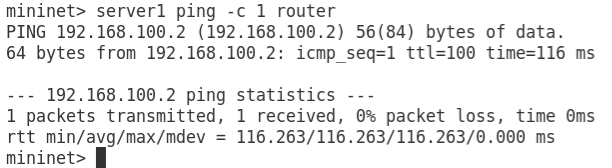
\includegraphics[width=\textwidth]{3}
	\caption{ping result}
\end{figure}
\begin{figure}[htbp]
	\centering
	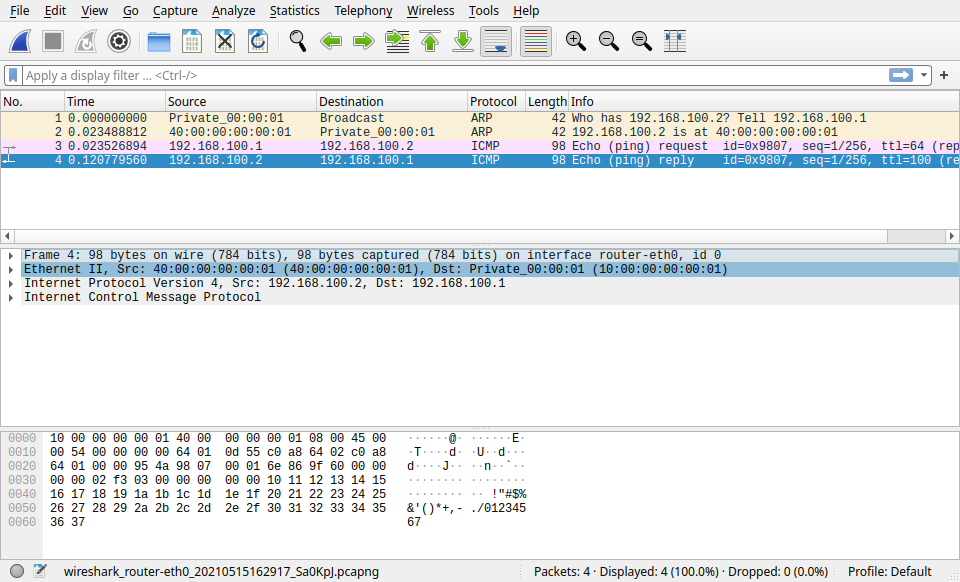
\includegraphics[width=\textwidth]{4}
	\caption{wireshark capture result}
\end{figure}

\subsubsection{TTL expire}
command: server1\# ping -c 1 -t 1 router \\
result:
\begin{figure}[htbp]
	\centering
	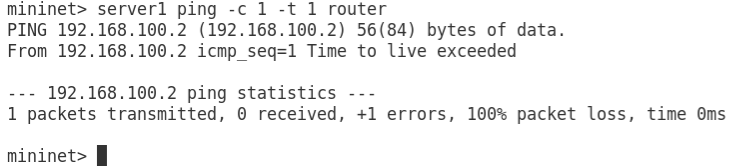
\includegraphics[width=\textwidth]{5}
	\caption{ping result}
\end{figure}
\begin{figure}[htbp]
	\centering
	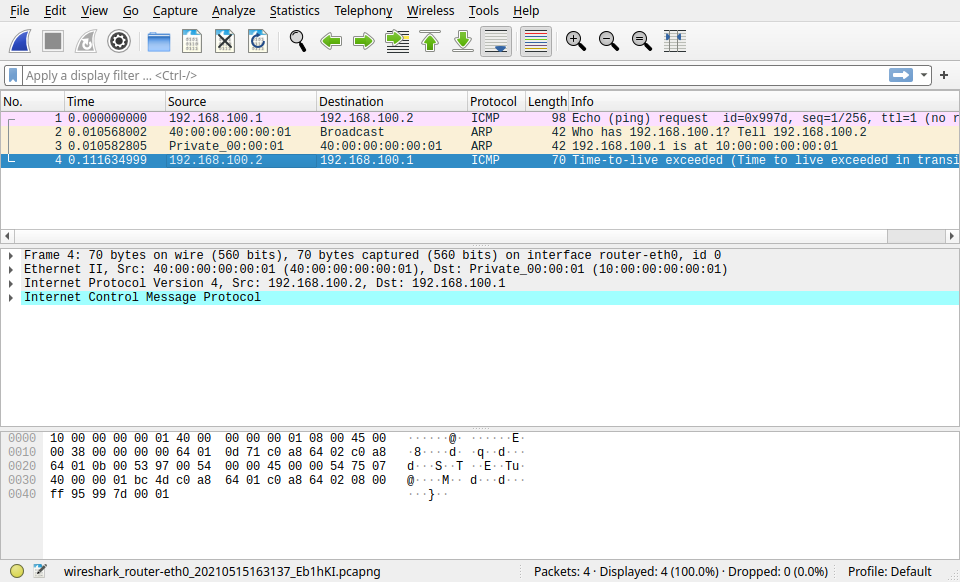
\includegraphics[width=\textwidth]{6}
	\caption{wireshark capture result}
\end{figure}

\newpage
\subsubsection{Destination network unreachable}
In order to generate destination network unreachable error with a ping request from server1, I added an entry to start\_mininet.py:
\lstinputlisting[style=python]{8.py}
command: server1\# ping -c 1 172.16.1.1 \\
result:
\begin{figure}[htbp]
	\centering
	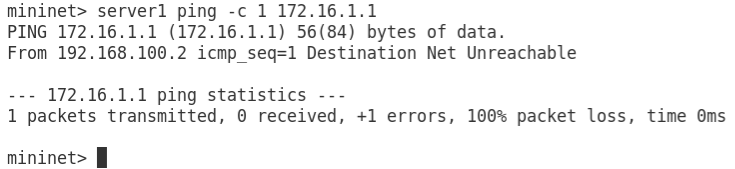
\includegraphics[width=\textwidth]{7}
	\caption{ping result}
\end{figure}
\begin{figure}[htbp]
	\centering
	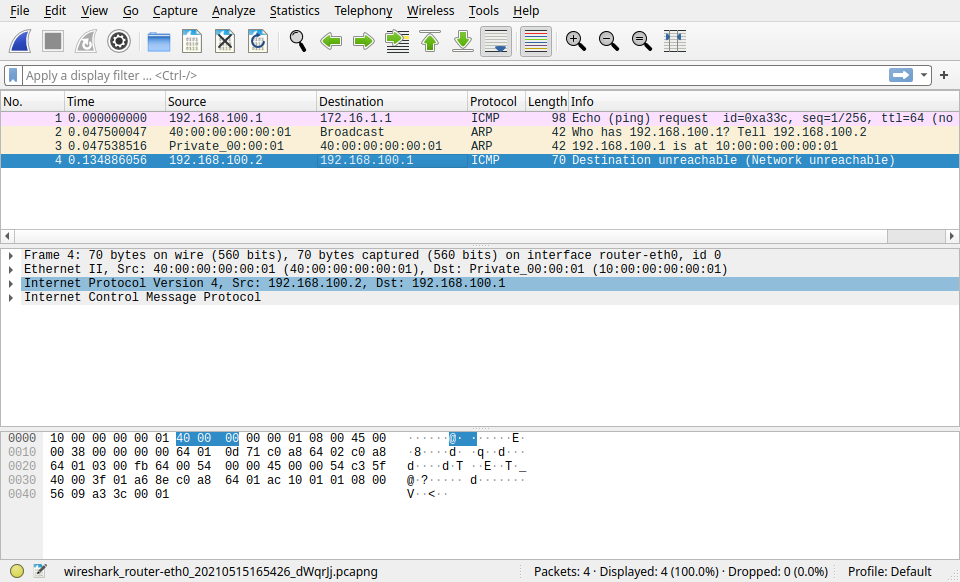
\includegraphics[width=\textwidth]{8}
	\caption{wireshark capture result}
\end{figure}

\newpage
\subsubsection{Traceroute}
Lastly I tested my implementation with traceroute command:
\begin{figure}[htbp]
\centering
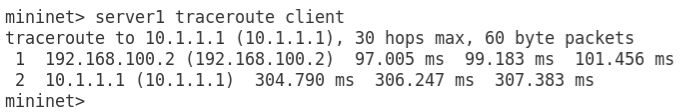
\includegraphics[width=\textwidth]{9}
\caption{traceroute test result}
\end{figure}
\\It turned out fine! Besides, it is worth mentioning that I didn't use -N option, which means my program can efficiently handle a large number of packets in a very short time.

\section{Summary}
\begin{itemize}
	\item Knowing how to use tools effectively will greatly enhance working efficiency;
	\item always keep your code simple and clear, or you have to reconstruct it before you can add new functions;
	\item English reading and writing skills are important.
\end{itemize}

\end{document}